\section{Construction and Visualization of Feature Surfaces}
\label{sec:visualization}
%
The flamelets extracted as profiles in the previous step can directly be used
by combustion researchers for statistical analysis of the whole flame front.
%
We will not go into detail about this here, as it is outside the scope of this
work.
%
In this section, we present a novel visualization based on the feature points
extracted on the profiles that augments the statistical approach with a visual
analysis component.
%

%
The model parameters $x_l$, $x_m$ and $x_r$ (see \cref{fig:models}) describe
three classes of feature points on the profiles: \emph{minimum} (min),
\emph{maximum} (max) and \emph{inflection point} (infl).
%
% Using the position and direction of the profile lines, we transform those
% feature points into points in space. These points can describe a feature surface
% through the points of steepest slope, local maximum function values, etc.,
% depending on which feature point class is chosen, revealing more about the
% scalar fields than a simple isosurface can.
% 
These feature points span feature surfaces of the respective variables that can
have physical or chemical significance.
%
For example, the surfaces of maximum heat release or maximum concentration of a
radical are sometimes used as alternative definitions of the flame surface.
%
The feature surfaces of maximum and minimum temperature bound the flame front
and indicate the flame thickness.
%
Investigating the shapes and local distances of these surfaces gives insight
into the local combustion process and how it is affected by turbulent flow.
%
We now describe the construction of those feature surfaces and their
visualization.
%
% This section describes techniques to visualize feature surfaces -- i.e.,
% surfaces of interest -- of the DNS data. For this, by having the above
% introduced Sigmoid and Gaussian model as sparse DNS data representation,
% different classes of feature points w.r.t. the flame simulation can be revealed.
% These classes are \emph{maximum} $t_{max}$, \emph{inflection point} $t_t$, and
% \emph{minimum} $t_{min}$. They are related to the model's functions, which
% Figure~\ref{fig_models} illustrates. Based on that, we introduce the
% construction of feature points for all models of the DNS data.
%
% \begin{figure}[t!]
%     \centering
%  	\resizebox{240pt}!{\includegraphics{figures/models.pdf}}
% 	\caption{\label{fig_models}%
% 		Feature point classes: minimum $t_{\min}$, inflection point $t_{t}$,
% 		and maximum $t_{\max}$ of Sigmoid and Gaussian model.
% 	}
% \end{figure}
%
%
\subsection{Feature Point Construction}
%
The positions of the feature points on the profiles represent
intersections with the corresponding feature surfaces in the original data.
%
By shifting the anchor points $\vp_i$ onto the intersections with a specific
feature surface, we transform them to a feature point set sampling this surface
(see \cref{fig:featurepoints}, left).
%
Considering a profile line $\vp(t)$ anchored on the flame surface $S$, the
position of a feature point $\vp(t_f)$ with $f \in \{\text{min}, \text{max},
\text{infl}\}$ is given by
%
\begin{equation*}
	\vp(t_{f})=\vp + t_f \cdot \vn.
\end{equation*}
% with $t_{n}$ being the normalization
% \begin{equation}
% 	t_{n}= - \frac{ \vp \cdotp \vr }{ ||\vr||^2 }
% 		+ \sqrt{   
% 			(\vp\cdotp\vr)^2
% 			- \frac{ ||\vp||^2-\tau^2 }{ ||\vr||^2 }
% 		}. \nonumber
% \end{equation}
%
% It is based on the model distance $\tau$ and the model's feature point
% distance $t_f$, as illustrated in Figure~\ref{fig_pointcloud} (middle).
%
Here, $t_f$ is the shift value for the respective feature surface given by
$x_l$, $x_m$ or $x_r$ of the corresponding profile.
%
For example, the shift values $t_{\textnormal{max}}$ for the surface of maximum heat
release are obtained by the $x_m$ values of the heat release profiles.
%
Having constructed these feature points is the first step in constructing a
feature surface, which we detail in the following section.
%
% \begin{figure}[t]
%     \centering
%  	\resizebox{250pt}!{\includegraphics{figures/pointcloud.pdf}}
% 	\caption{\label{fig_pointcloud}%
% 	Revealing a feature point set based on flame surface and data models: (left)
% 	Initial flame surface $S$ and its profile lines $\vp_i(t),
% 	i=1,\dots,n$ given by point $\vp_i$ and its direction vector
% 	$\vr_i$. (middle) A potential configuration of parametrized Gaussian
% 	models for each profile line. Please note that the model's abscissa is
% 	aligned with the related direction vector. For illustration, the maximum
% 	$t_{max_i}$ is emphasized for each model. Of course, also further classes of
% 	feature points as well as the Sigmoid model could be considered. (right)
% 	With the aid of the profile line and model, the position of the feature
% 	point, e.g. the maximum, in space can be reveled by
% 	$\vp_i(t_{max_i})$. All those feature points define a point set of
% 	feature points. By considering a potential surface running through all
% 	feature points a feature surface, here a maximum surface $S_{t_{max}}$
% 	(light red), is found. }
% \end{figure}

%
\subsection{Feature Surface Construction}
%
Remember that during the transformation to the sparse representation, an
isosurface mesh $M$ representing the flame surface $S$ was extracted.
%
The profile lines were seeded at vertices of this mesh.
%
For each vertex $\vp_i$ on the flame surface mesh we therefore know the position
of a point on the feature surface $S_f$ by the corresponding shift value
$t_{fi}$ and the direction of the profile line $\vn_i$
(\cref{fig:featurepoints}, left).
%
% Revealing a feature surface is a non-trivial task due to reasons of ambiguity:
% obviously, an infinite number of surfaces can be fitted to the point set. Thus,
% the construction issue ends up in a selection issue, i.e., selecting one
% relevant surface. To solve this selection issue, we subsequently exploit the
% knowledge about the relation between the feature point set and the flame
% surface.
%
% \begin{figure}[t]
%     \centering
%  	\resizebox{245pt}!{\includegraphics{figures/featurecontourconstruction.pdf}}
% 	\caption{\label{fig_featurecontourconstruction}%
% 	Relations between flame surface $S$, flame mesh $M$, profile lines
% 	$\vp_i(t)$, and feature point set $\vp_i(t_f)$: (left) Initial
% 	flame surface $S$, its profile lines $\vp_i(t), i=1,\dots,n$ given by
% 	points $\vp_i$ and direction vectors $\vr_i$, and a mesh $M$
% 	of the flame surface, given by the points $\vm_j,j=1,\dots,k$ (light
% 	blue) and its edges (black lines) based on Marching Cubes algorithm. (right)
% 	In addition, the relations between a feature point set and the profile lines
% 	are illustrated: start points $\vp_i$ are not aligned/related to a
% 	vertex points $\vm_j$ of flame surface mesh $M$, i.e., start points
% 	and vertices have different positions. }
% \end{figure}
%
% To construct a feature surface from a feature point set, we use our knowledge
% about the relation between the feature point set and the flame surface.
% Note that the flame surface $S$ equates to an isosurface of the data. An iso-
% surface mesh $M$ of the flame surface was extracted during the transformation to
% the sparse representation. A feature surface $S_f$ does not equate to an iso-
% surface. Therefore a mesh $M_f$ representing the feature surface is not as
% easily extracted from the data. However, the position of a point on the feature
% surface is known for every point $\vp_i$ by the corresponding shift value
% $t_{f_i}$ and the direction of the profile $\vr_i$
% (Figure~\ref{fig:featurepoints} (left)).
%
% Therefore, a mesh $M$, discretely representing the flame surface $S$, can be
% revealed by using Marching Cubes \cite{Lorensen:1987:CG}. Furthermore, a feature
% surface $S_f$ does not equate to an isosurface. Thus, a mesh $M_{f}$,
% discretely representing the feature surface $S_f$, cannot be revealed using,
% e.g., Marching Cubes.
%
The idea is to transform the flame surface mesh $M$ into a feature surface mesh
$M_{f}$ representing the feature surface.
%
%This can be done by exploiting the relations between the feature points set and
%the flame surface mesh.
\begin{figure}[t!]
	\centering
	% \def\svgwidth{0.8\textwidth}
	% \import{figures/}{featurepoints.pdf_tex}
	\begin{tikzpicture}[
    thick,
    surface/.style={gray, very thick},
    feature/.style={red!50!white},
    arrow/.style={-latex, very thick},
    point/.style={draw=black, fill=yellow},
    mesh/.style={fill=cyan},
    fpoint/.style={fill=red}
    ]

    \newcommand*{\rzero}{30}
    \newcommand*{\rone}{30}
    \newcommand*{\rtwo}{0}
    \newcommand*{\rthree}{-45}
    \newcommand*{\rfour}{-80}

    \newcommand*{\rmone}{15}
    \newcommand*{\rmtwo}{-22}
    \newcommand*{\rmthree}{-70}

    \newcommand*{\defcoords}{%
        \coordinate (p0) at (-0.75, 1.9);
        \coordinate (p1) at (-0.5, 1.2);
        \coordinate (p2) at (0, 0);
        \coordinate (p3) at (-0.3, -1.2);
        \coordinate (p4) at (-1, -1.6);

        \coordinate (m1) at (-0.205, 0.6);
        \coordinate (m2) at (-0.08, -0.6);

        \coordinate (r0) at (\rzero:0.35cm);
        \coordinate (r1) at (\rone:0.3cm);
        \coordinate (r2) at (\rtwo:0.7cm);
        \coordinate (r3) at (\rthree:0.5cm);
        \coordinate (r4) at (\rfour:0.4cm);

        \coordinate (rm1) at (\rmone:0.45cm);
        \coordinate (rm2) at (\rmtwo:0.65cm);

        \coordinate (pf0) at ($(p0) + (r0)$);
        \coordinate (pf1) at ($(p1) + (r1)$);
        \coordinate (pf2) at ($(p2) + (r2)$);
        \coordinate (pf3) at ($(p3) + (r3)$);
        \coordinate (pf4) at ($(p4) + (r4)$);

        \coordinate (pmf1) at ($(m1) + (rm1)$);
        \coordinate (pmf2) at ($(m2) + (rm2)$);
    }

    \begin{scope}[scale=1.5]
        \defcoords{}

        \draw[surface] plot[smooth] coordinates{(p0) (p1) (m1) (p2) (m2) (p3) (p4)};
        % \foreach \p in {pf1, pf2, pf3}{
        %     \begin{scope}
        %         \clip (\p) circle (0.5cm);
        %         \draw[surface, feature] plot[smooth] coordinates{(pf0) (pf1) (pmf1) (pf2) (pmf2) (pf3) (pf4)};
        %     \end{scope}
        % }
        \node[surface, above left] at (p0) {$S$};
        % \node[surface, feature, above] at (pf0) {$S_f$};

        \begin{scope}[rotate=\rone, shift=(p1)]
                \draw[black] (-1.5, 0) -- (1.5, 0);
                \draw plot[smooth, tension=0.5] coordinates{
                    (-1.5, 0.05) (-1, 0.1) (-0.5, 0.2) (0, 0.4) (0.3, 0.5)
                    (0.5, 0.45) (1, 0.25) (1.5, 0.15)
                };
                \draw[dashed] (0.3, 0.5) -- (0.3, 0);
                \draw[point, fpoint] (0.3, 0.5) circle (0.5mm);
        \end{scope}
        \begin{scope}[rotate=\rtwo, shift=(p2)]
                \draw[black] (-1.5, 0) -- (1.5, 0);
                \draw plot[smooth, tension=0.5] coordinates{
                    (-1.5, 0.03) (-1, 0.07) (-0.5, 0.15) (0, 0.3)
                    (0.5, 0.47) (0.7, 0.5) (1, 0.45) (1.5, 0.31)
                };
                \draw[dashed] (0.7, 0.5) -- (0.7, 0);
                \draw[point, fpoint] (0.7, 0.5) circle (0.5mm);
                \draw[point, fill=black] (0.7, 0) circle (0.5mm);
        \end{scope}
        \begin{scope}[rotate=\rthree, shift=(p3)]
                \draw[black] (-1.5, 0) -- (1.5, 0);\draw plot[smooth, tension=0.5] coordinates{
                    (-1.5, 0.05) (-1, 0.1) (-0.5, 0.22) (0, 0.35)
                    (0.5, 0.5) (1, 0.35) (1.5, 0.27)
                };
                \draw[dashed] (0.5, 0.5) -- (0.5, 0);
                \draw[point, fpoint] (0.5, 0.5) circle (0.5mm);
                \draw[point, fill=black] (0.5, 0) circle (0.5mm);
        \end{scope}

        \draw[arrow] (p1) -- ++(\rone:1cm);% node[below right] {$\vr_1$};
        \draw[arrow] (p2) -- ++(\rtwo:1cm) node[below] {$\vr_i$};
        \draw[arrow] (p3) -- ++(\rthree:1cm);% node[below] {$\vr_3$};

        \foreach \i in {1, 2, 3}{
            \draw[point] (p\i) circle (0.5mm);
            \draw[point, fill=black] (pf\i) circle (0.5mm);
        }
        \foreach \i in {1, 2}{
            \draw[point, mesh] (m\i) circle (0.5mm);
            \node[gray] at (pmf\i) {\LARGE\textbf{?}};
        }
        % \node[below left=0.15cm and -0.3cm of p1] {$\vp_1$};
        \node[below left] at (p2) {$\vp_i$};
        % \node[left=0.07cm of p3] {$\vp_3$};

        % \node[right=0.2cm of pf1] {$\vp'_1$};
        \node[below left=0.05cm and 0.1cm of pf2] {$\vp'_i$};
        % \node[below=0.15cm of pf3] {$\vp'_3$};

        \node[left] at (m2) {$\vm_j$};
    \end{scope}

    \begin{scope}[scale=1.5, xshift=3cm]
        \defcoords{}

        % \draw[surface] plot[smooth] coordinates{(p0) (p1) (m1) (p2) (m2) (p3) (p4)};
        % \draw[surface, feature] plot[smooth] coordinates{(pf0) (pf1) (pmf1) (pf2) (pmf2) (pf3) (pf4)};
        \node[above left] at (p0) {$M$};
        \node[red, above] at (pf0) {$M_f$};
        \draw[black] plot coordinates{(p0) (p1) (m1) (p2) (m2) (p3) (p4)};
        \draw[red] plot coordinates{(pf0) (pf1) (pmf1) (pf2) (pmf2) (pf3) (pf4)};

        \draw[arrow] (p1) -- ++(\rone:1cm);
        \draw[arrow] (p2) -- ++(\rtwo:1cm);
        \draw[arrow] (p3) -- ++(\rthree:1cm);


        \draw[arrow, gray] (m1) -- ++(\rmone:1cm);% node[right] {$\vr'_1$};
        \draw[arrow, gray] (m2) -- ++(\rmtwo:1cm) node[right] {$\vr'_j$};
        % \draw[arrow] (p3) -- ++(\rthree:1cm);

        \foreach \i in {1, 2, 3}{
            \draw[point] (p\i) circle (0.5mm);
            \draw[point, fill=black] (pf\i) circle (0.5mm);
        }
        \foreach \i in {1, 2}{
            \draw[point, mesh] (m\i) circle (0.5mm);
            \draw[point, gray, fill=gray] (pmf\i) circle (0.5mm);
        }
        % \node[below left=0.15cm and -0.3cm of p1] {$\vp_1$};
        \node[left] at (p2) {$\vp_i$};
        % \node[above left=-0.15cm and 0.07cm of p3] {$\vp_3$};
        % \node[below left] at (m1) {$\vm_1$};
        \node[left] at (m2) {$\vm_j$};
        % \node[gray, below left=0.0cm and -0.2cm of pmf1] {$\vm'_1$};
        \node[gray, below left=-0.2cm and 0.1cm of pmf2] {$\vm'_j$};

    \end{scope}

\end{tikzpicture}
	\tikzset{external/export=false}
	\caption{Construction of feature points and feature mesh (simplified \ac{2D}
	representation).
	%
	Left: Construction of feature points (\protect\tikz\protect\draw[thick,
	fill=black] circle [radius=0.8mm];) by shifting anchor points
	(\protect\tikz\protect\draw[thick, fill=white] circle [radius=0.8mm];)
	along their normals.
	%
	% Left: Feature points are constructed by shifting the anchor points $\vp_i$
	% on the flame surface $S$ along their normal vectors $\vn_i$ by amount
	% $t_f$ taken from the model parameters (here, $x_m$ of a Gaussian model).
	% %
	% The resulting points $\vp_i(t_{f i})$ are located on feature surface $S_f$.
	%
	Right: Positions for the other mesh vertices on the feature mesh
	(\protect\tikz\protect\draw[thick, fill=gray, draw=gray] circle
	[radius=0.8mm];) are obtained via diffusion of the known normals and shift
	values.
	%
	% Right: Feature mesh $M_f$ is constructed from flame surface mesh $M$ by
	% shifting all vertices along their corresponding directions by their
	% corresponding values of $t_f$.
	% %
	% Normals and shift values for mesh points $\vm_j$ are obtained
	% by diffusion (gray arrows and dots).
	}
	\label{fig:featurepoints}
	\tikzset{external/export=true}
\end{figure}
%

%
The simplest way to implement this transformation would be to move the vertices
$\textbf{m}_j$ of $M$ along the corresponding normal vectors $\vn_j$ to a
related feature point, given by the shift value $t_{fj}$.
%
Unfortunately, the values for $t_f$ and $\vn$ are not known everywhere on the
mesh, but only at vertices where profile lines have been seeded (see
\cref{sub:seeding,fig:featurepoints}).
%
% Unfortunately, this is not possible, since the flame mesh $M$ and the profile
% lines $\vp(t)=\vp+ t \cdotp \vr$ are mutually not aligned,
% as Figure~\ref{fig_featurecontourconstruction} illustrates.
%
% \begin{figure}[t]
%     \centering
%  	\resizebox{240pt}!{\includegraphics{figures/diffusion.pdf}}
% 	\caption{\label{fig_diffusion}%
% 	Sharing information which belongs to the profile lines with the surface mesh
% 	vertices: (a) Embedding the start points $\vp$ of profile lines into
% 	the flame mesh $M$ by re-meshing triangle $T \in M$. (b) Update of the
% 	feature vector $\textbf{i}(\textbf{m})$ of vertex $\vm \in M$ (blue)
% 	is iteratively computed by considering the adjacent (orange edges) vertices
% 	(blue) and points (yellow). (c) Several iteration update steps for a value
% 	$s(\vm) \in \vi(\vm)$ for vertices (blue) depending on
% 	values of the points (yellow). For simplicity, cross sections are shown. }
% \end{figure}
%
Thus, the first step of the transformation is to approximate this information
for the other vertices.
%

%
We use a diffusion-driven approach to obtain directions $\vn'_j$ and shift
values $t'_{fj}$ for each mesh vertex from the original $\vn_i$ and $t_{fi}$.
%
For this, we fix the original values at the vertices corresponding to points
$\vp_i$ and diffuse them over the rest of the mesh until convergence.
%
Different diffusion methods can be used to obtain results of varying smoothness.
%
For simplicity, we use an explicit weighted averaging scheme, iteratively
replacing the values at each vertex with the sum of its immediate neighbors,
weighted with the neighbor's inverse distance.
%
After this process has finished, we have directions and shift values for each
vertex $\vm_j$ to obtain approximated feature mesh vertices $\vm'_j$ (gray
dots in \cref{fig:featurepoints}, right).
%
This process is a preprocessing step that has to be performed only once before
visualization and does not further impede performance.
%
% Thus, the first step of transformation has to be to map required information
% onto the flame mesh $M$. This information are the directions of the profile line
% $\vr_i=(r_{x_i},r_{y_i},r_{z_i})^T$ and the feature distance values
% $t_{f_i}$, which gives in total a 4D information vector
% $\vi=(r_{x_i},r_{y_i},r_{z_i},t_f)^T$ that needs to be related with the
% mesh.
% %
% For this, our approach uses a diffusion-driven method to share information over
% mesh $M$: Let $T$ be a triangle -- given by the points
% $\vm_a,\vm_b,$ and $\vm_c$ -- of mesh $M$. Then, the
% triangle's centroid $\vp_{a,b,c}$ is given by $\vp_{a,b,c}=1/3 ~
% \cdotp (\vm_a+\vm_b+\vm_c)$.
% %
% Please remember that $\vp$ is start point of a profile line
% $\vp(t)$, sent out from flame surface. Such start point $\vp$ will
% be related to a triangle $T$ (i) if it is placed in the same voxel and (ii) if
% it is the closest to a triangle's centroid, i.e.,
% $||\vp-\vp_{a,b,c}|| \rightarrow \min$ for all triangles of the
% same voxel is fulfilled. Please note that only a number of zero or one points
% $\vp$ might be related with a triangle $T$, since only one profile line
% per voxel has been seeded.
% %
% Next, each triangle $T$ of flame mesh $M$, which is related with point
% $\vp$, is re-meshed by replacing the triangle
% $(\vm_a,\vm_b,\vm_c)$ by triangles
% $(\vm_a,\vp,\vm_c)$,
% $(\vm_a,\vp,\vm_b)$, and
% $(\vm_b,\vp,\vm_c)$. This way $\vp$ is embedded and
% becomes a part of flame mesh $M$, as Figure~\ref{fig_diffusion}(a) illustrates.

% What remains is to iteratively share the information vectors
% $\vi(\vp)$ of embedded points $\vp$ with the vertices
% $\vm$ of mesh $M$: At first, the information vectors $\vi$ of
% vertices $\vm$ are initialized as zero-vectors:
% $\vi(\vm)=\v0$. Then, as shown by
% Figure~\ref{fig_diffusion}(b), an update of each scalar value $s(\vm_i)
% \in \vi(\vm_i)$
% %w.r.t. information vector $\vi$
% is computed for each vertex $\vm_i$. For this, adjacent vertices
% $\vm_j$ and adjacent points $\vp_l$ in mesh $M$ are considered:
% %
% \begin{equation}
% 	s(\vm_i) =
% 		\frac{1}{J+L} 
% 		\sum^J s(\vm_j) \cdotp \Omega(||\vm_i-\vm_j||))
% 		+ \sum^L s(\vp_l) \cdotp \\\Omega(||\vm_i-\vp_l||))
% 		\text{,}\nonumber
% \end{equation}
% with $\Omega(r)=1/r$. By continuously repeating this computation for each vertex
% $\vm$, the updates for $s \in \vi$ eventually converges.
% Figure~\ref{fig_diffusion} (c) points this out.
% %
% After this process is done, an information vector $\textbf{i}_i=(\vr_i,
% t_{f_i})$ is available for each vertex $\textbf{m}_i$ of the flame mesh $M$. It
% describes direction $\vr_i$ and distance $t_{f_i}$ to a related feature
% point. By moving the vertices with $\textbf{m}_{i_f} = \textbf{m}_i +
% \frac{t_{f_i}}{t_{{n}_i}} \cdotp \vr_i$, the flame mesh $M$ is
% transformed into a feature mesh $M_f$, which gives a piecewise-linear
% approximation of feature surface $S_f$. In that manner, the initially mentioned
% selection issue is solved.
%
%Laufzeit/Limitationen
%
\subsection{Feature Surface Visualization}
%
\begin{figure}[p]
    \centering
    \setlength\figurewidth\textwidth
    \begin{tikzpicture}[
    every node/.style={node distance=0,
                       font=\small},
    label/.style={yshift=1mm},
    row label/.style={anchor=base west, xshift=-1cm, font=\normalsize}
]
    % \node (gui) {
    %     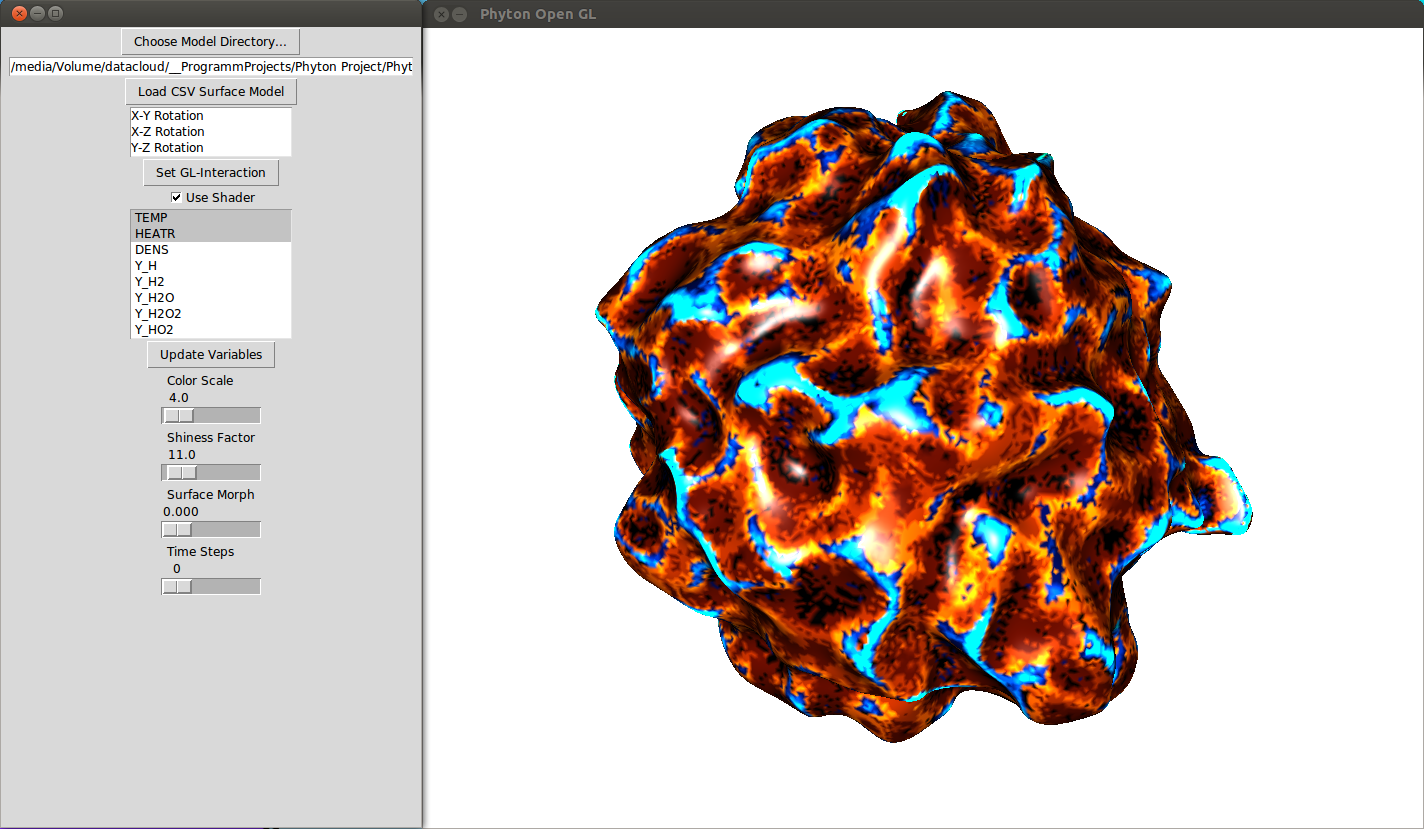
\includegraphics[width=0.5\figurewidth]{figures/sr_gui.png}
    % };

    \matrix[matrix of nodes,] (cs) {
        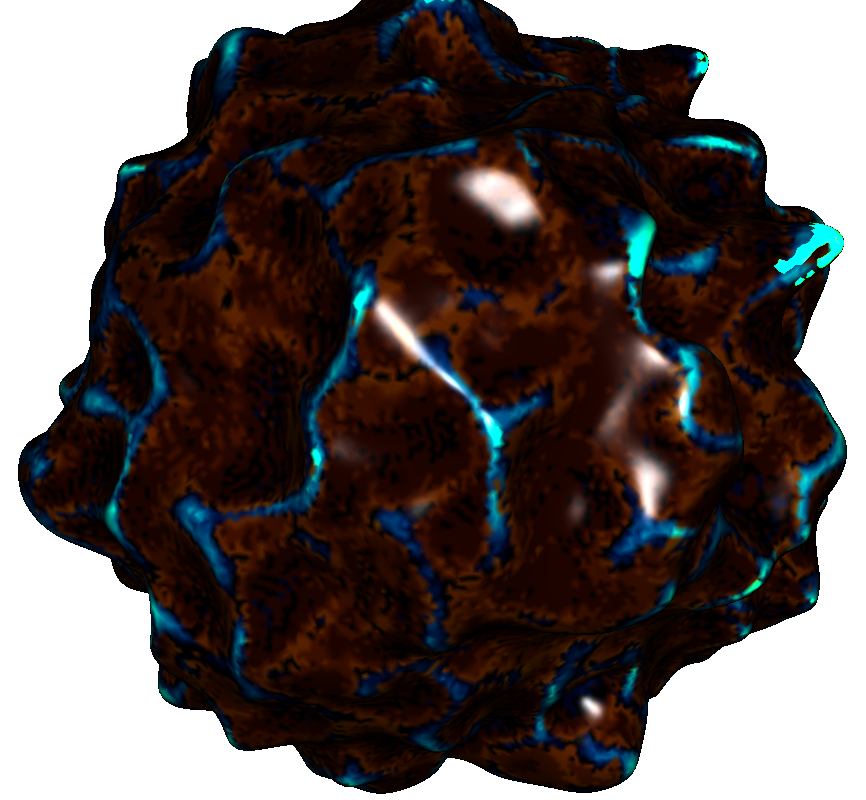
\includegraphics[width=0.22\figurewidth]{figures/sr_colorscale_1.png} &
        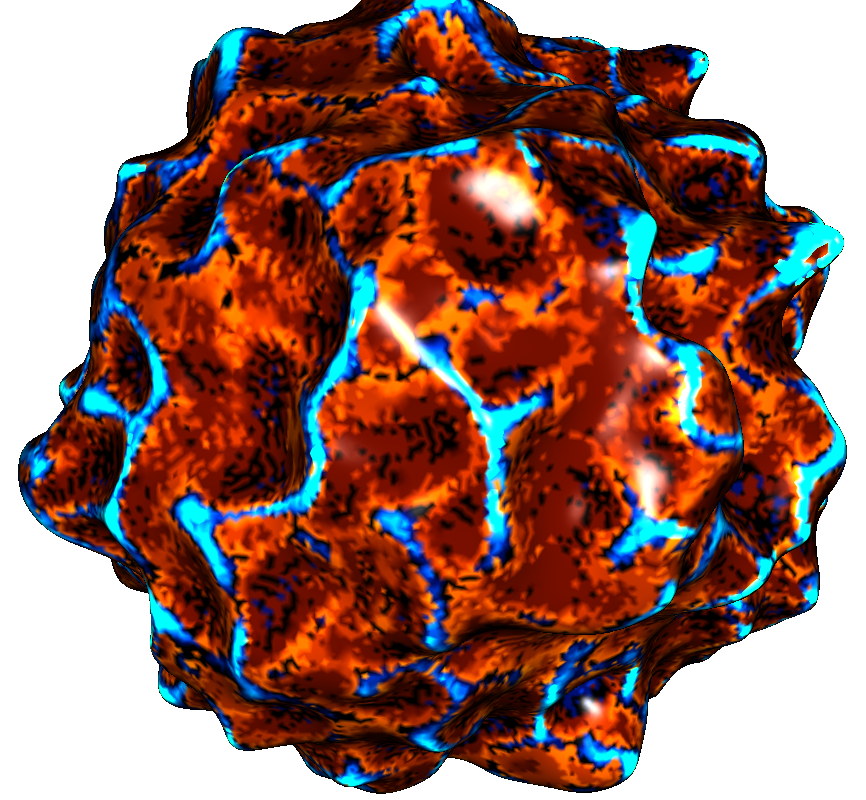
\includegraphics[width=0.22\figurewidth]{figures/sr_colorscale_2.png} &
        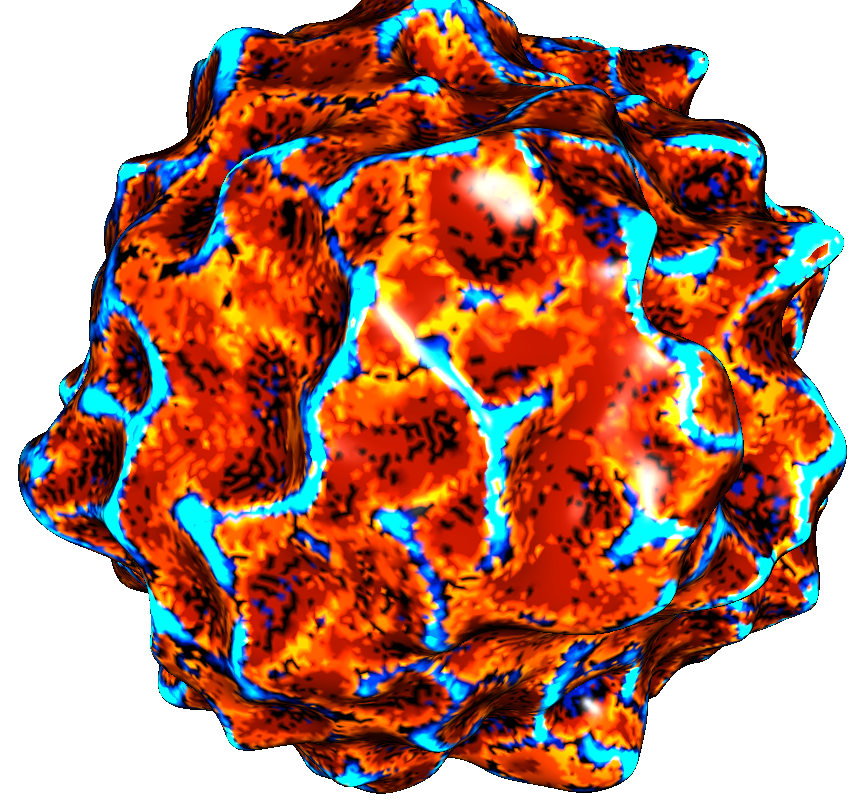
\includegraphics[width=0.22\figurewidth]{figures/sr_colorscale_3.png} \\
    };
    \node[label, below=of cs-1-1] {$u_1=1$};
    \node[label, below=of cs-1-2] {$u_1=2.5$};
    \node[label, below=of cs-1-3] {$u_1=4$};

    % \draw[thick] ([xshift=-1cm]cs.south west) -- (cs.south east);
    \node[row label, at=(cs.north west)] {color scale};
    \node[left=of cs] {
        \rotatebox{90}{$t^\textnormal{TEMP}_\textnormal{infl}$
                       vs. $t^\textnormal{HEATR}_\textnormal{max}$}
    };

    \matrix[matrix of nodes, below=1cm of cs] (morph) {
        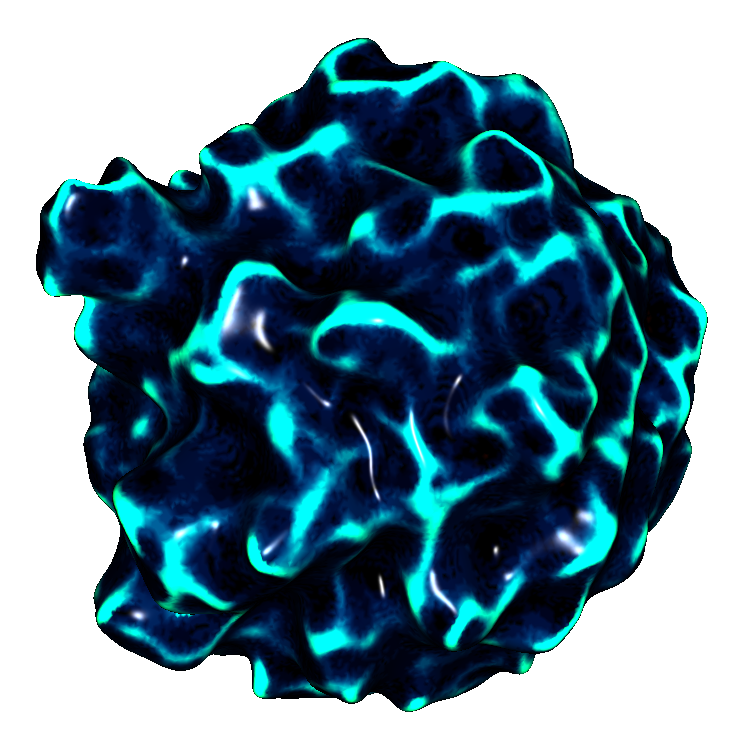
\includegraphics[width=0.22\figurewidth]{figures/sr_morphing_1.png} &
        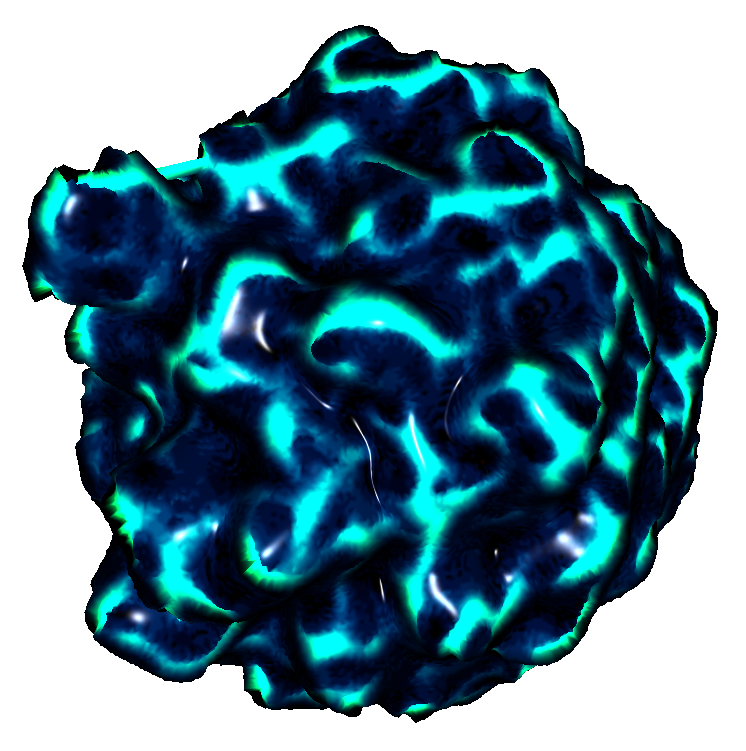
\includegraphics[width=0.22\figurewidth]{figures/sr_morphing_2.png} &
        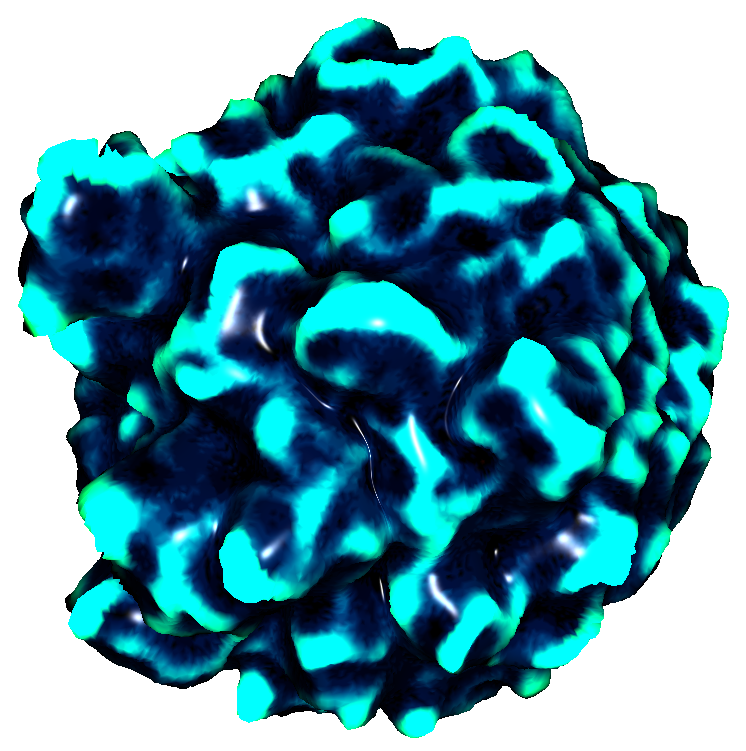
\includegraphics[width=0.22\figurewidth]{figures/sr_morphing_3.png} \\
    };
    \node[label, below=of morph-1-1] {$u_2=0$};
    \node[label, below=of morph-1-2] {$u_2=1$};
    \node[label, below=of morph-1-3] {$u_2=2$};

    % \draw[thick] ([xshift=-1cm]morph.south west) -- (morph.south east);
    \node[row label, at=(morph.north west)] {morphing};
    \node[left=of morph] {
        \rotatebox{90}{$t^\textnormal{HEATR}_\textnormal{max}$
                       vs. $t^{\ce{H2O2}}_\textnormal{max}$}
    };

    \matrix[matrix of nodes, below=1cm of morph] (time) {
        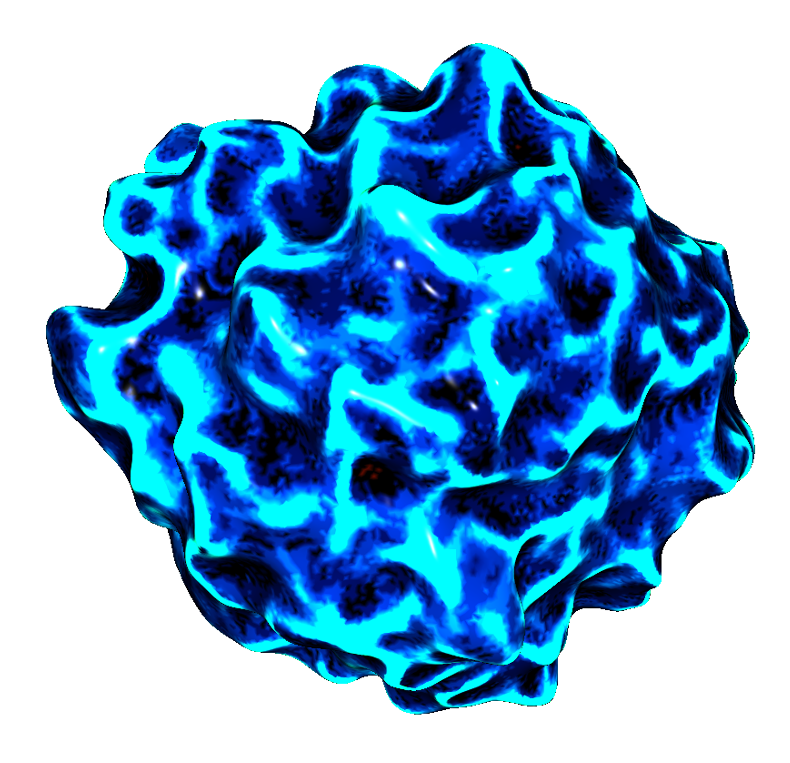
\includegraphics[width=0.22\figurewidth]{figures/sr_time_1_1.png} &
        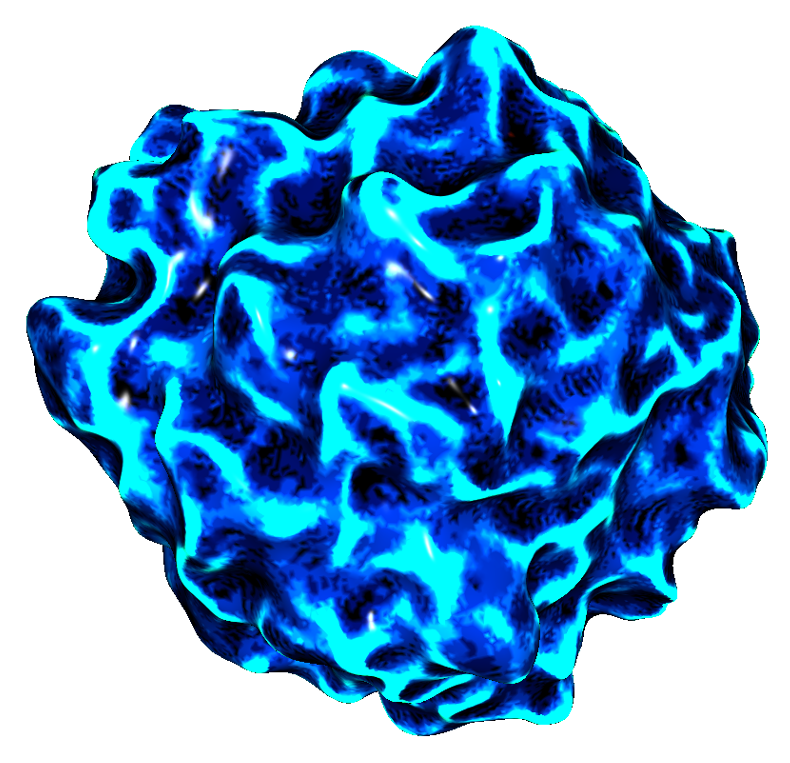
\includegraphics[width=0.22\figurewidth]{figures/sr_time_1_2.png} &
        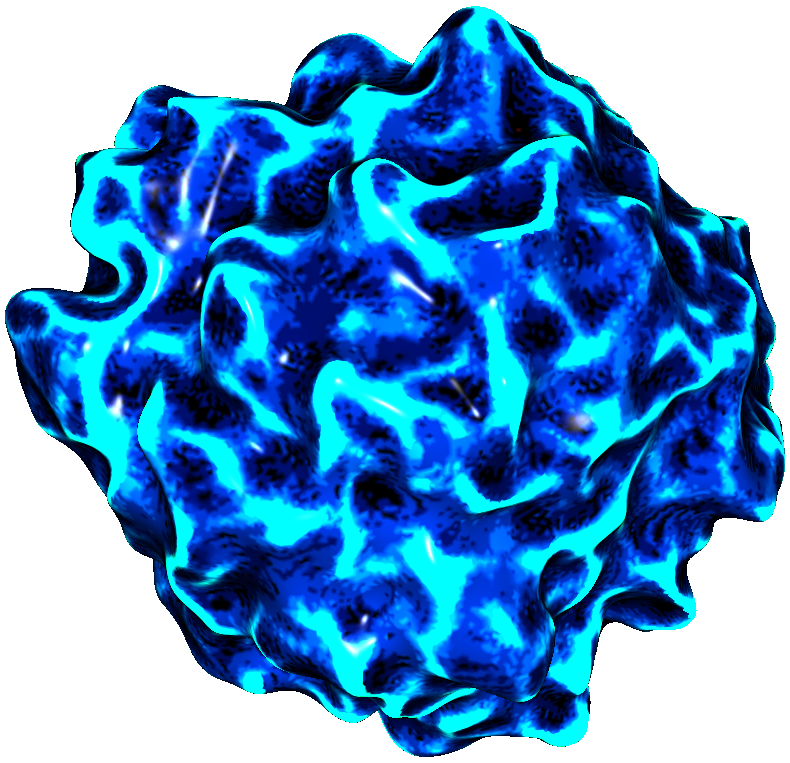
\includegraphics[width=0.22\figurewidth]{figures/sr_time_1_3.png} \\
        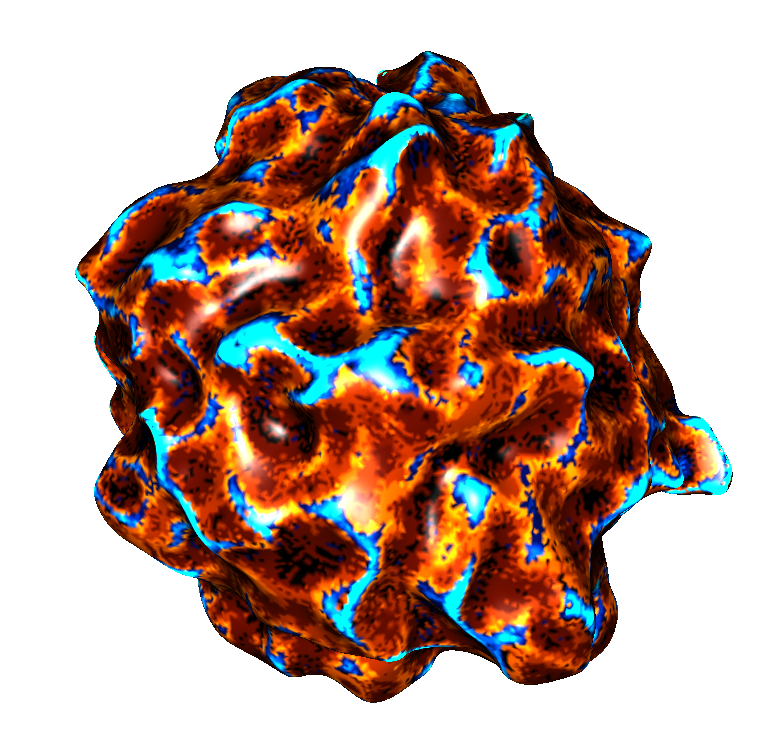
\includegraphics[width=0.22\figurewidth]{figures/sr_time_2_1.png} &
        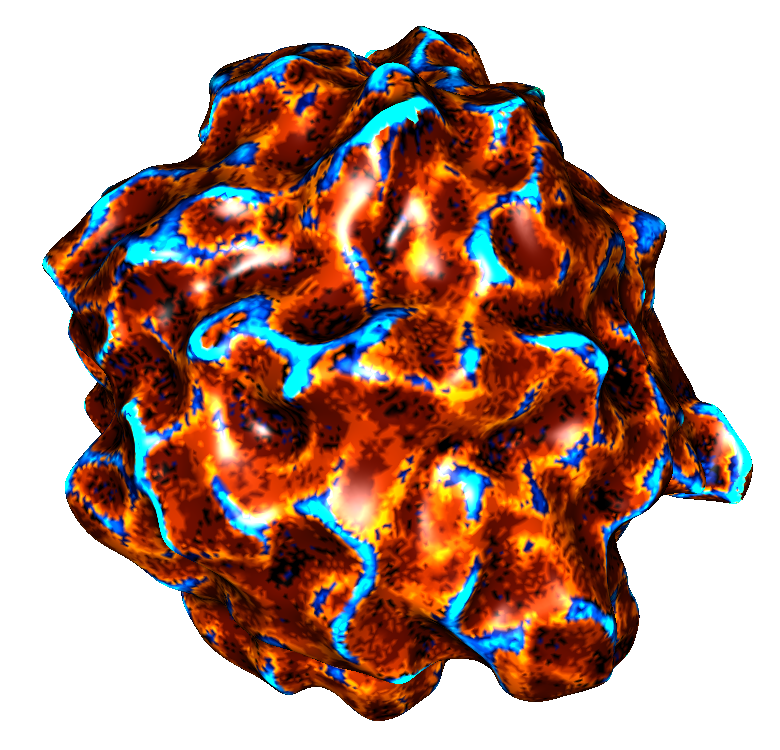
\includegraphics[width=0.22\figurewidth]{figures/sr_time_2_2.png} &
        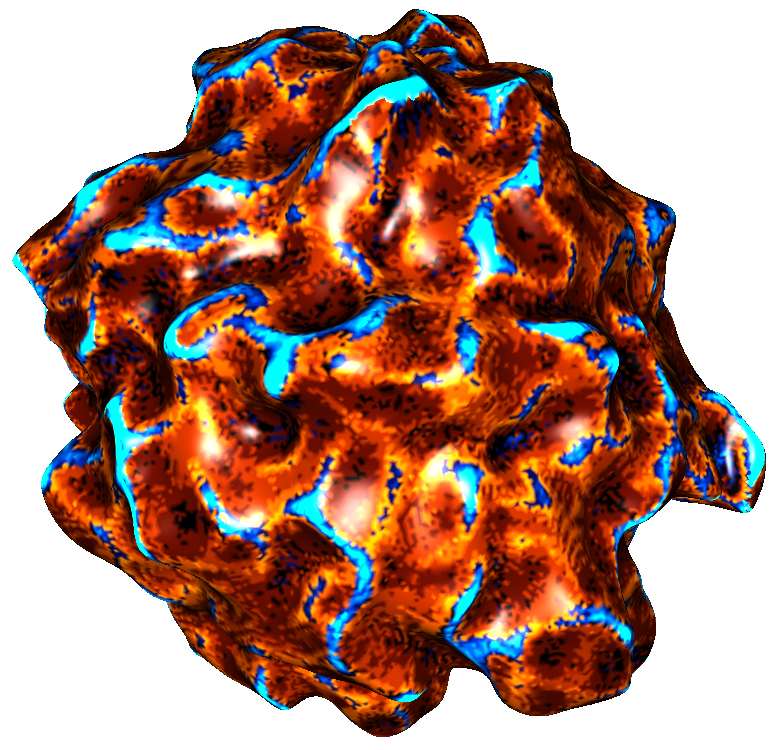
\includegraphics[width=0.22\figurewidth]{figures/sr_time_2_3.png} \\
        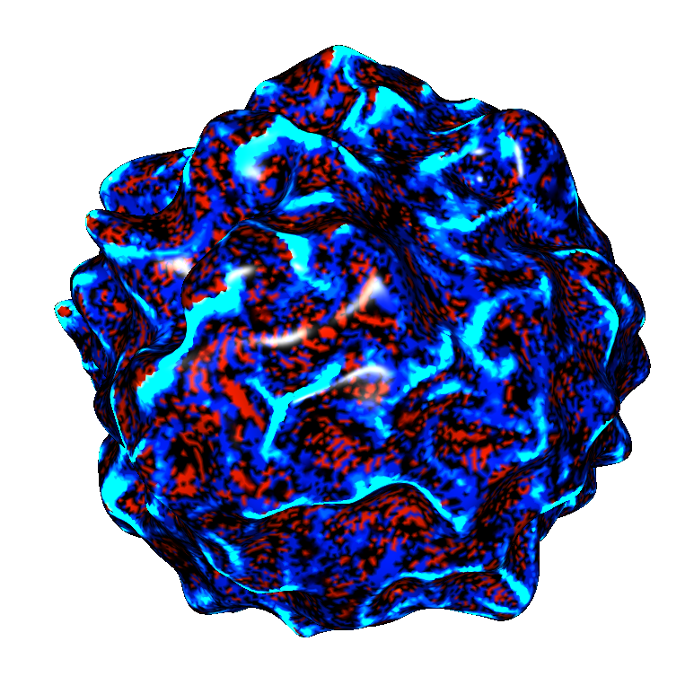
\includegraphics[width=0.22\figurewidth]{figures/sr_time_3_1.png} &
        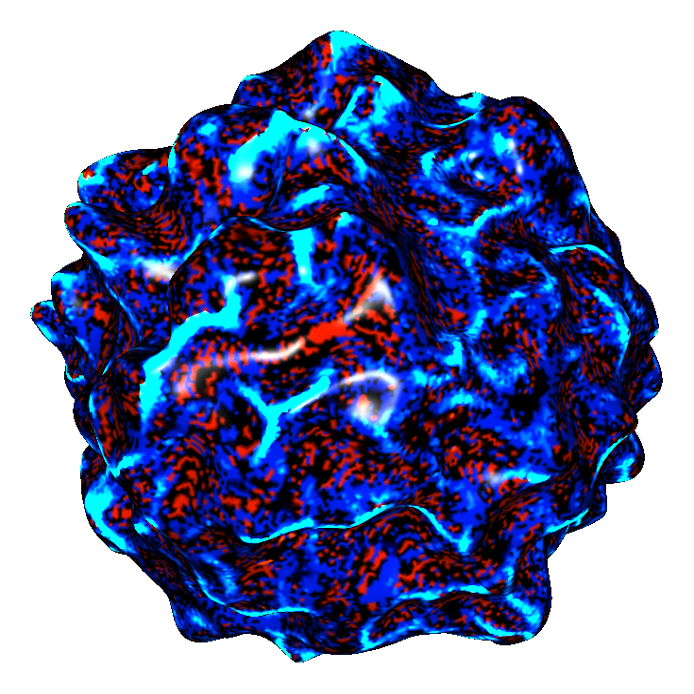
\includegraphics[width=0.22\figurewidth]{figures/sr_time_3_2.png} &
        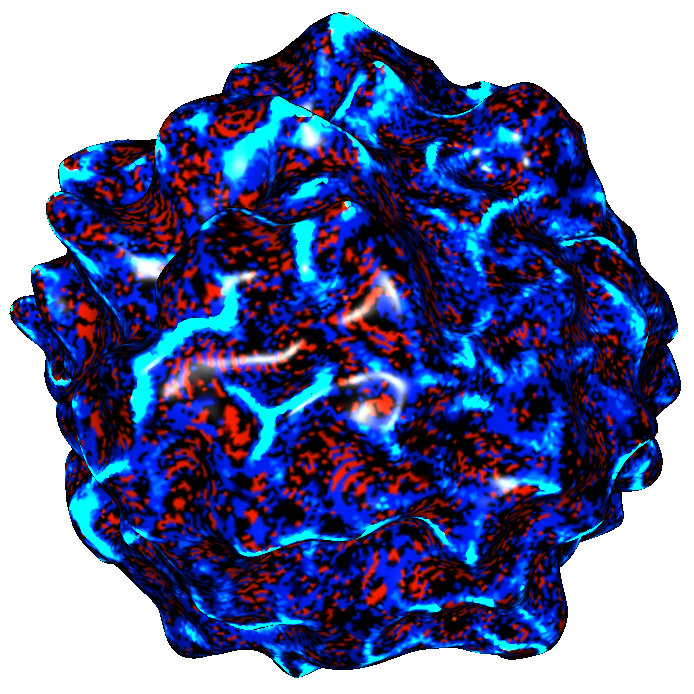
\includegraphics[width=0.22\figurewidth]{figures/sr_time_3_3.png} \\
    };
    \node[label, below=of time-3-1] {time step 1};
    \node[label, below=of time-3-2] {time step 4};
    \node[label, below=of time-3-3] {time step 8};

    \node[row label, at=(time.north west)] {time steps};

    \node[left=of time-1-1] {
        \rotatebox{90}{$t^\textnormal{HEATR}_\textnormal{max}$
                       vs. $t^{\ce{H2O2}}_\textnormal{max}$}
    };
    \node[left=of time-2-1] {
        \rotatebox{90}{$t^\textnormal{TEMP}_\textnormal{infl}$
                       vs. $t^\textnormal{HEATR}_\textnormal{max}$}
    };
    \node[left=of time-3-1] {
        \rotatebox{90}{$t^\textnormal{TEMP}_\textnormal{infl}$
                       vs. $t^{\ce{O}}_\textnormal{max}$}
    };
\end{tikzpicture}
    \caption{Prototype of visual analysis tool for feature meshes showing dataset
        \textsc{Hydrogen}.
        \Todo[inline]{add circles marking interesting features}
    }
    \label{fig_contourmeshvis}
\end{figure}
%
\begin{figure}[t]
	\begin{captionbeside}{Graphical user interface of our prototype visual analysis tool.
		\label{fig:gui}}
		\setlength\figurewidth{0.6\textwidth}
		\begin{tikzpicture}[
    every node/.style={inner sep=0, outer sep=0}
]
    \node (img) {
        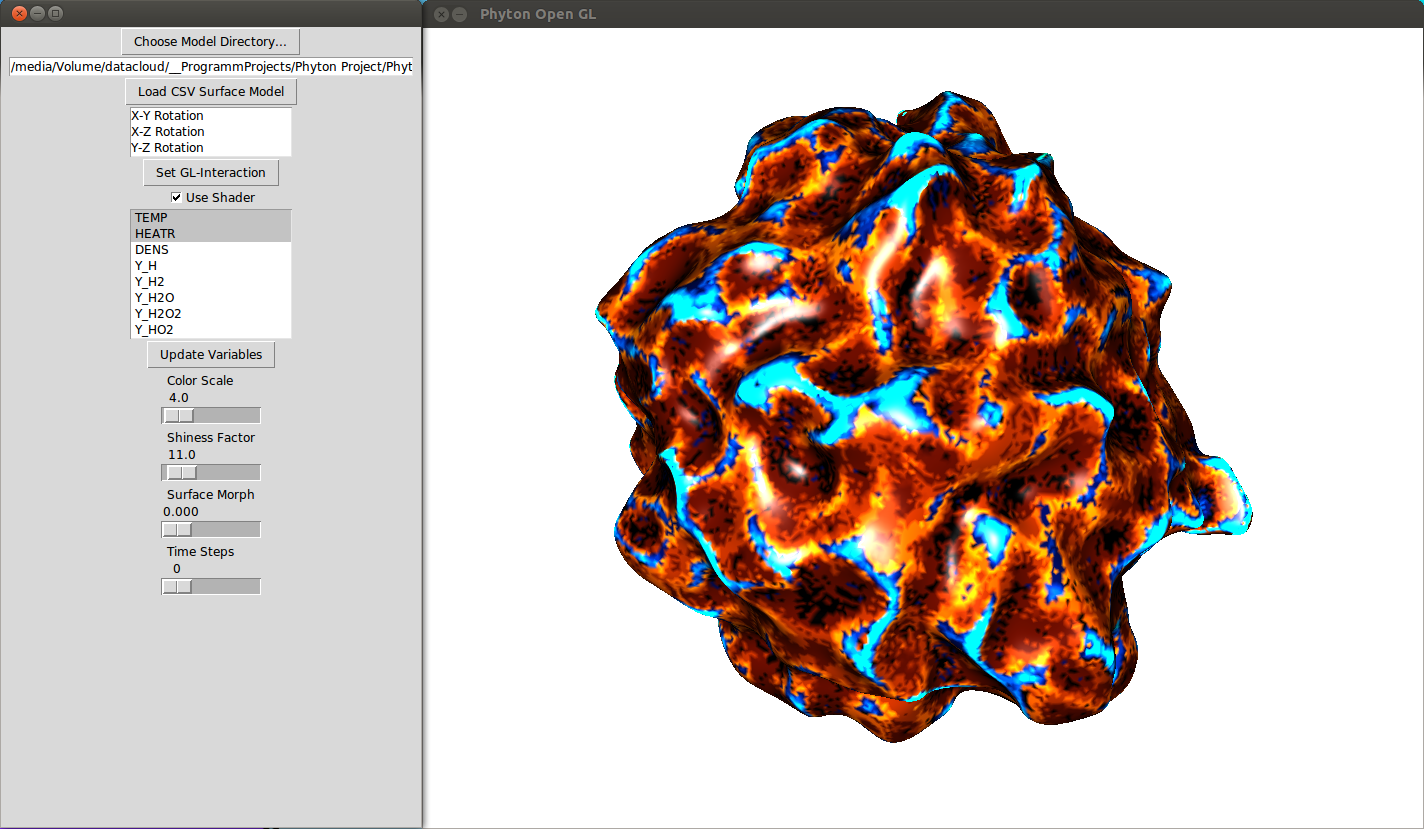
\includegraphics[width=\figurewidth]{figures/sr_gui.png}
    };
\end{tikzpicture}
	\end{captionbeside}
\end{figure}
%
With a method to construct feature surfaces from the sparse representation, we
can now visualize these surfaces in different ways.
%
Domain experts want to visually examine the feature surfaces, and investigate
the differences between feature surfaces of different variables or feature point
classes.
%
In the following, we introduce our approach for enabling such an analysis task.
%
% Up to here, feature meshes from DNS data have been constructed. Now an
% appropriate visualization concept is required to allow for the visual
% analysis of characteristic flame features and their relations.
% %
% Such a mesh encodes semantical information about the simulation. Thus, it is a
% relevant source of information for domain experts. Domain experts want
% to visually examine two properties: first, distances between feature meshes of
% different variables of the DNS data. Second, the shape of the meshes themselves.
% %
% In the following, we introduce an interactive visualization and analysis
% concept for feature meshes.
%
%The related concepts are subsequent discussed.
%----------------------------------------------
\subsubsection{Pairwise Distance Visualization}
%
Given two different feature surfaces, a comparative visualization must highlight
differences and similarities.
%
In the context of flamelet analysis, the differences between surfaces along
the normal direction is most interesting.
%
We therefore propose a visualization to explore pairwise distances between
feature surfaces.
%

%
A visualization of distances between feature surfaces of two different variables
must allow for quickly identifying regions of small or large distance, as well
as the distances' orientation.
%
We achieve this by displaying the local distance
between two feature surfaces color-coded on the flame surface mesh.
%
This mesh serves as a neutral and common base for comparison, which is related
to both feature surfaces.
%

%
As mentioned, corresponding vertices $\vm_f^V$ and $\vm_f^W$ of two
different feature meshes can be obtained from the vertex $\vm$ by shifting
it by two different values $t_f^V$ and $t_f^W$ along the local normal direction
$\vn'$.
%
Thus, the distance between the vertices is simply the difference between the two
shift values.
%
This distance is computed for each vertex and linearly mapped onto a color map. 
%
% The mapping is given by
% %
% \begin{equation}
% 	\begin{array}{ll}
% 		1 & \text{if } u_1 \cdotp d + 0.5 > 1 \text{,}\\
% 		0 & \text{if } u_1 \cdotp d + 0.5 < 0 \text{,}\\
% 		u_1 \cdotp d + 0.5 & \text{ else.}\\
% 	\end{array}
% \end{equation}
% %
% This mapping ensures that $d=0$ is always mapped to the center of the color map.
%

%
We use a color map adapted to our application:
%
black for values near zero (the meshes intersect), red to yellow for growing
positive distances (one mesh is outside of the other locally), and blue to cyan
for negative distances (the opposite applies).
%

%
We introduce parameter $u_1$ as a scaling factor for adjusting the color
contrast and controlling how much of the data is mapped inside the displayed
color range and how much is clamped to the maximum/minimum color.
%
This enables a quick visual search for both extreme difference values (by
choosing a low value for $u_1$), or an overview of areas with positive or
negative difference values (by choosing a high value for $u_1$).
%
The color scale and the effect of varying parameter $u_1$ are shown in
\cref{fig_contourmeshvis}.
\Todo{adjust reference after updating figure}
%

% Let $M^{v}_{f}$ and $M^{w}_{f}$ feature meshes for two variables $v$ and $w$ of
% DNS data w.r.t. the same feature class $f$. Let $M$ the related flame mesh, and
% $t_\phi=t_f/t_{n}$.
% %
% For vertex $\vm \in M$, the related points on the feature meshes
% $M^{v}_{f}$ and $M^{w}_{f}$ are given by:
% \begin{equation}
% 	%\vm_f^v=\vm+ \frac{t^v_f}{t^v_{n}} \cdotp \vr \in M^{v}_{f} \text{ and }
% 	%\vm_f^w=\vm+ \frac{t^w_f}{t^w_{n}} \cdotp \vr \in M^{w}_{f}. \nonumber
% 	\vm_f^v=\vm+ t^v_\phi \cdotp \vr \in M^{v}_{f}
% 	\text{ and }
% 	\vm_f^w=\vm+ t^w_\phi \cdotp \vr \in M^{w}_{f}\text{.}
% 	\nonumber
% \end{equation}
% %
% The Euclidean distance $d(\vm_f^{v,w})$ between points $\vm_f^v$
% and $\vm_f^w$ is:
% \begin{eqnarray}
% 	d(\vm_f^{v,w})
% 	= || \vm_f^v-\vm_f^w ||
% 	= || (\vm + t^v_\phi \cdotp \vr)
% 	- (\vm+ t^w_\phi \cdotp \vr) ||
% 	= || t^v_\phi -t^w_\phi ||\text{.}\nonumber
% \end{eqnarray}
% %
% From this, the signed Euclidean distance $d_s(\vm_f^{v,w})$ follows as
% \begin{equation}
% 	d_s(\vm_f^{v,w}) = t^v_\phi - t^w_\phi. \nonumber
% \end{equation}
% %
% To visualize difference values $d_s$, they are mapped onto a $[0,1]$ range
% as well as a related color map $(r,g,b)$ given by:
% %
% \begin{eqnarray}
% 	u_1 \cdotp (d_n,d_n^2,0), \text{ if } d_n < 0.5, \nonumber\\ 
% 	u_1 \cdotp (0,d_n^2 - 0.5,d_n -0.5), \text{  else}, \nonumber
% \end{eqnarray}
% %
% \begin{equation}
% 	\text{with}~~
% 	d_n = \frac{0.5 \cdotp |d_s|}{\max(|d_s|)} + a \text{, and } 
% 	a = 0 \text{ if } d_s < 0 \text{,} ~ a = 0.5 \text{ else,} \nonumber
% \end{equation}
% and $u_1$ being a scaling factor steered by the user.
% %address a review comment
% %----
% With this factor, the user adjust the color contrast which enables a quick visual search for
% both extrem diference values (by choosing a low value for scaling factor)
% or an overview of the zero-crossings over the surface (black bands on the surface, i.r.,
% blue to red transition by choosing a large value for scaling factor.
% %----
% Of course, further color
% maps can be used. However, this color map is adopted to our application:
% intersections between the meshes are given by $d_n=0.5$ (\emph{black});
% $d_n<0.5$ (\emph{blue} to \emph{light-blue}) means that one mesh is in front of
% the other; $d_n>0.5$ (\emph{red} to \emph{yellow}) means that the opposite
% applies. Finally, the approach visualizes the Euclidean differences for the two
% feature surface meshes $M^{v}_{f}$ and $M^{w}_{f}$ by color coding the
% differences $d(\vm_f^{v,w})$ as vertex colors for the related vertices
% $\vm$ of the flame mesh $M$. The color-coding and the use of parameter
% $u_1$ is illustrated by Figure~\ref{fig_contourmeshvis}(b).

% Using the flame mesh for color coding differences of the feature surface meshes
% w.r.t. two data set variables is reasonable because: (i) feature meshes and
% flame meshes are mutually related and (ii) the flame mesh gives a data-driven
% and neutral shape that can be used for analysis purposes.
% %
% This way, the user can focus on finding color-driven interesting difference properties of the features meshes,
% instead of being deflected by, e.g., different shapes.
%----------------------------------------------------------------------------------
\subsubsection{Feature Mesh Visualization}
%
We use standard computer graphics techniques to render the feature surfaces.
%
The distance values are mapped to the mesh as vertex colors, and Phong shading
is used to enhance the perception of surface curvature.
%
Larger specular highlights improve the curvature perception but obstruct the
view on the mesh color. We therefore let the user control the specular
reflectance factor to suit their needs.
%
% The feature surface meshes can be visualized by using standard computer graphics
% illumination and shading techniques. For this, the direction vector $\vr$
% is interpreted as surface normal and vertex normal, respectively, and a Phong
% shading is applied. Figure~\ref{fig_contourmeshvis} shows a couple of examples
% w.r.t. the color-coded mesh shading.
% %Address review comment
% %------
% It can be seen that we also provide to steer the Phong's shininess.
% The shininess visually encodes curvature information, thus
% a larger value eases the investigation of the surface structure. Coevally, it
% dominates the color, i.e., a large value makes it difficult to see the color-coded
% differences anymore. Thus, the shininess can be steered in increasing as well as decreasing direction.
%------

%
To allow for the investigation of the feature meshes' shapes, we provide a
user-controlled linear morphing between the flame surface mesh $M$ and the two
chosen feature meshes $M^{V}_{f}$ and $M^{W}_{f}$.
%
A parameter $u_2 \in [0, 2]$ steers the morphing, showing the original flame
surface $M$ for $u_2 = \num{0}$, the first feature surface $M^{V}_{f}$ for $u_2
= \num{1}$ and $M^{W}_{f}$ for $u_2 = \num{2}$ (\cref{fig_contourmeshvis}).
\Todo{adjust reference after updating figure}
%
The morphing itself is trivial.
%
Since the corresponding vertices between all the meshes are known
and their topology is identical, they just have to be linearly translated as the
value of $u_2$ changes.
%
% \todo{neccessary?} Letting the user continuously control the value of $u_2$ lets them control the
% speed of the morphing and allows for reversing the direction at any time. This
% allows for a better understanding of the relations between the meshes, compared
% to an animation of the morphing.

%
Finally, we enable the user to quickly slide through the different time steps
and investigate the temporal behavior of the feature surfaces and their
relations.
%
This allows for a quick interactive visual analysis that would have been
impossible to achieve on the original raw simulation data, due to the large
number and storage size of time steps.
%

% In addition, a morphing between the flame mesh $M$ and the feature meshes for
% two variables $M^{v}_{f}$ and $M^{w}_{f}$ is defined. A vertex $\vm(u_2)$
% of a mesh for this morphing is given by:
% %
% \begin{equation}
% 	\vm(u_2)=
% 		\begin{cases}
% 			\vm + u_2 \cdotp t^v_\phi \cdotp \vr
% 				& \mbox{if } u_2 \leq 1, \\
% 			u_2 \cdotp \vr \cdotp t^w_\phi - \vr \cdotp t^v_\phi
% 				& \mbox{else. }
% 		\end{cases} \nonumber
% \end{equation}
% %
% By steering the parameter $u_2$, the user is able to visually investigate the
% differences of the shape between all three meshes: $u_2=0$ gives $M$, $u_2=1$
% gives $M^{v}_{f}$, and $u_2=2$ gives $M^{w}_{f}$.
% Figure~\ref{fig_contourmeshvis}(c) depicts this.
%------------------

% As proof of concept, a prototype has been implemented using MatLab for
% performing the transformation to the sparse representation, and using Python
% with Tkinter, PyGame, and Python-OpenGL for the visual analysis tool. The user
% interface can be seen in Figure~\ref{fig_contourmeshvis} (top).
%